%\documentclass{article}
%\usepackage{tikz,pgfplots}
%\usepackage[pdftex,active,tightpage]{preview}
%\begin{document}
%\begin{preview}
%%%%%%%%%%%%%%%%%%%%%%%%%%%%%%
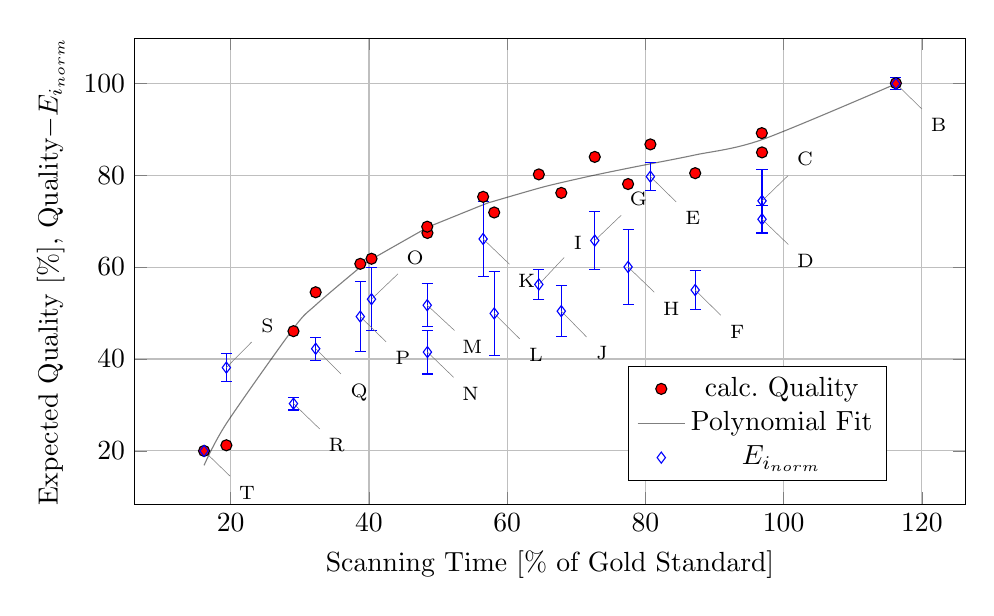
\begin{tikzpicture}

\begin{axis}[%
    xmajorgrids,
    ymajorgrids,
	width=\linewidth,
	height=0.618\linewidth,
    %scale only axis,
    %xmin=0,xmax=110,
    %ymin=0,ymax=110,
    %axis y line = left,
	xlabel={Scanning Time [\%\ of Gold Standard]},%
	ylabel={Expected Quality [\%], Quality$-E_{i_{norm}}$}%
	]

% Protocols
\addplot [ fill=red, only marks, mark = *]
	coordinates{
		(16.14,20)
		(19.37,21.2284)
		(29.08,46.0522)
		(32.29,54.5201)
		(38.75,60.7072)
		(40.37,61.8107)
		(48.46,67.4167)
		(48.43,68.7811)
		(58.12,71.8724)
		(56.52,75.28)
		(67.83,76.1345)
		(64.58,80.1592)
		(77.49,78.0612)
		(72.67,83.9645)
		(87.20,80.4284)
		(80.72,86.6889)
		(96.87,84.9458)
		(96.84,89.1421)
		(116.24,100)
};

% Line plot
\addplot [smooth, solid, semitransparent]
	coordinates{
		(16.14,16.8548)
		(19.37,25.9575)
		(29.08,46.6567)
		(32.29,51.7347)
		(38.75,59.9714)
		(40.37,61.6854) 
		(48.46,68.6146)
		(48.43,68.6305) 
		(56.52,73.5452)
		(58.12,74.3455)
		(64.58,77.1605)
		(67.83,78.3754)
		(72.67,80.0091)
		(77.49,81.5005)
		(80.72,82.4599)
		(87.20,84.3973)
		(96.87,87.719)
%		(96.87,87.719)
		(116.24,99.8565)
};

\addplot [ color=blue, only marks, mark=diamond ]
plot [ error bars/.cd, y dir=both, y explicit ]
    coordinates{
	( 16.14,20.0000) +- (0,0)      % T
	( 19.37,38.1358) +- (0,3.1135) % S
	( 29.08,30.2919) +- (0,1.3958) % R
	( 32.29,42.2255) +- (0,2.5278) % Q
	( 38.75,49.2247) +- (0,7.6789) % P
	( 40.37,53.0181) +- (0,6.8507) % O 
	( 48.46,41.5079) +- (0,4.7824) % N  
	( 48.43,51.6990) +- (0,4.7110) % M
	( 58.12,49.9058) +- (0,9.1839) % L
	( 56.52,66.1100) +- (0,8.1635) % K
	( 67.83,50.4137) +- (0,5.5671) % J
	( 64.58,56.2138) +- (0,3.2329) % I
	( 77.49,60.0243) +- (0,8.0805) % H
	( 72.67,65.7727) +- (0,6.2214) % G
	( 87.20,55.0069) +- (0,4.1882) % F
	( 80.72,79.6708) +- (0,3.0107) % E
	( 96.87,70.4018) +- (0,3.0863) % D
	( 96.87,74.3991) +- (0,6.8125) % C
	(116.24,99.8987) +- (0,1.3487) % B
};
	
\pgfplotsset{every axis legend/.append style={at={(0.75,0.1)},anchor=base}}

\legend{calc.\ Quality, Polynomial Fit, $E_{i_{norm}}$}

% \draw [<-] (axis cs:97.87,74.3991) -- (axis cs:99.87,74.3991) node [anchor=text] {\tiny C}; 
% \draw [<-] (axis cs:97.87,70.4018) -- (axis cs:99.87,70.4018) node [anchor=text] {\tiny D};
% \draw [<-] (axis cs:81.72,79.6708) -- (axis cs:82.72,79.6708) node [anchor=text] {\tiny E};
% \draw [<-] (axis cs:78.49,60.0243) -- (axis cs:79.49,60.0243) node [anchor=text] {\tiny H};
% \draw [<-] (axis cs:65.58,56.2138) -- (axis cs:66.58,56.2138) node [anchor=text] {\tiny I};
% \draw [<-] (axis cs:49.43,51.6990) -- (axis cs:51.43,51.6990) node [anchor=text] {\tiny M};
% \draw [<-] (axis cs:49.46,41.5079) -- (axis cs:51.46,41.5079) node [anchor=text] {\tiny N};

%\tikzstyle{every pin}=[fill=white,draw=black,font=\tiny]
\tikzstyle{every pin}=[font=\scriptsize]
\node[coordinate, pin=below right:{B}] at (axis cs:116.24,99.8987) {}; % B
\node[coordinate, pin=above right:{C}] at (axis cs:96.87,74.3991) {}; % C
\node[coordinate, pin=below right:{D}] at (axis cs:96.87,70.4018) {}; % D
\node[coordinate, pin=below right:{E}] at (axis cs:80.72,79.6708) {}; % E
\node[coordinate, pin=below right:{F}] at (axis cs:87.20,55.0069) {}; % F
\node[coordinate, pin=above right:{G}] at (axis cs:72.67,65.7727) {}; % G
\node[coordinate, pin=below right:{H}] at (axis cs:77.49,60.0243) {}; % H
\node[coordinate, pin=above right:{I}] at (axis cs:64.58,56.2138) {}; % I
\node[coordinate, pin=below right:{J}] at (axis cs:67.83,50.4137) {}; % J
\node[coordinate, pin=below right:{K}] at (axis cs:56.52,66.1100) {}; % K
\node[coordinate, pin=below right:{L}] at (axis cs:58.12,49.9058) {}; % L
\node[coordinate, pin=below right:{M}] at (axis cs:48.43,51.6990) {}; % M
\node[coordinate, pin=below right:{N}] at (axis cs:48.46,41.5079) {}; % N  
\node[coordinate, pin=above right:{O}] at (axis cs:40.37,53.0181) {}; % O
\node[coordinate, pin=below right:{P}] at (axis cs:38.75,49.2247) {}; % P
\node[coordinate, pin=below right:{Q}] at (axis cs:32.29,42.2255) {}; % Q
\node[coordinate, pin=below right:{R}] at (axis cs:29.08,30.2919) {}; % R
\node[coordinate, pin=above right:{S}] at (axis cs:19.37,38.1358) {}; % S
\node[coordinate, pin=below right:{T}] at (axis cs:16.14,20.0000) {}; % T

\end{axis}

\end{tikzpicture}
%%%%%%%%%%%%%%%%%%%%%%%%%%%%%%
%\end{preview}
%\end{document}

%%%%%%%%%%%%%%%%%%%%%%%%%%%%%%
% plot erstellt mit MATLAB-File p:\\MATLAB\WideFieldScan/Paper/wfs_Compare2008c_ErrorPlot.m
% mit FromToTo = 1:5:1024
% sowie matlab2tikz
% Daten
%%%%%%%%%%Time =
%%%%%%%%%%  Columns 1 through 12
%%%%%%%%%%
%%%%%%%%%%   13.75   16.50   24.77   27.50   33   34.38   41.27   41.25   49.50   48.14   57.77   55
%%%%%%%%%%
%%%%%%%%%%  Columns 13 through 19
%%%%%%%%%%
%%%%%%%%%%   66   61.89   74.27   68.75   82.50   82.50   99.01
%MeanCumulativeError =
%
%  Columns 1 through 12
%
%   20.0000   38.1358   30.2919   42.2255   49.2247   53.0181   41.5079   51.6990   49.9058   66.1100   50.4137   56.2138
%
%  Columns 13 through 19
%
%   60.0243   65.7727   55.0069   79.6708   70.4018   74.3991   99.8987
%
%
%StandardDeviationofCumulativeError =
%
%  Columns 1 through 12
%
%         0    3.1135    1.3958    2.5278    7.6789    6.8507    4.7824    4.7110    9.1839    8.1635    5.5671    3.2329
%
%  Columns 13 through 19
%
%    8.0805    6.2214    4.1882    3.0107    3.0863    6.8125    1.3487
%%%%%%%%%%%%%%%%%%%%%%%%%%%%%%